\begin{frame}
\frametitle{Definition Baum}

\begin{columns}
\begin{column}{0.58\textwidth}

\only<1>{
    \begin{definition}
        Ein Baum ist eine ausdauernde und verholzende Samenpflanze mit einer dominierende Sprossachse, die durch sekundäres Dickenwachstum an Umfang zunimmt.
    \end{definition}
}
\only<2>{Nein Spass, jedes Kind weiß, dass das so nicht stimmt. In Wirklichkeit ist das ganz anders.}
\only<3->{
    \begin{definition}[Baum]
        %Ein \textbf{Baum} ist ein zusammenhängender, azyklischer Graph. Ein Graph, dessen Zusammenhangskomponenten Bäume sind, heißt \textbf{Wald}.
        zusammenhängender, azyklischer Graph
    \end{definition}
}
\only<4>{
    \begin{definition}[Wald]
        Graph, dessen Zusammenhangskomponenten Bäume sind
    \end{definition}
}
\only<5>{
    \begin{definition}[aufspannender Baum]
        Ein \textbf{aufspannender Baum} eines Graphen $G$ ist ein Baum, der alle Knoten von $G$ enthält.
    \end{definition}
}
\only<6>{
    \begin{definition}[Blatt]
        Ein Knoten eines Baums mit Grad 1 heißt \textbf{Blatt}.
    \end{definition}
}
\end{column}
\begin{column}{0.43\textwidth}
\only<1>{
\begin{figure}
    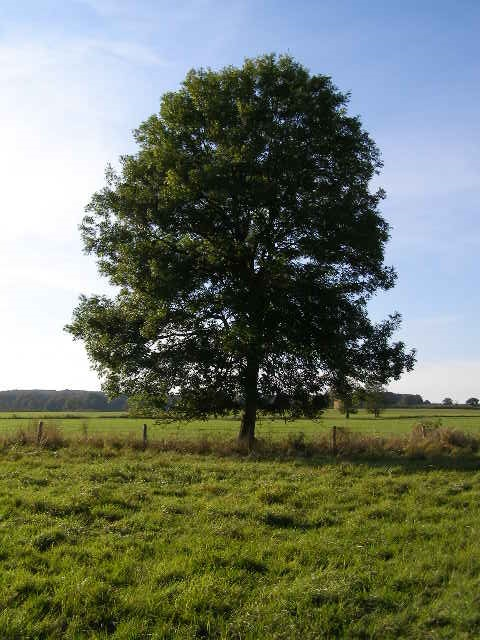
\includegraphics[width= \textwidth]{pictures/baum.jpg}
\end{figure}
}
\only<3> {
	\begin{figure}
		\begin{tikzpicture}[scale=1.3, auto,swap]
    % Draw a 7,11 network
    % First we draw the vertices
    \foreach \pos/\name in {{(0,0)/a}, {(1,1)/b}, {(3,1)/c},
                            {(0,-2)/d}, {(2,0)/e}, {(1,-1)/f}, {(3,-1)/g}}
        \node[vertex] (\name) at \pos {$\name$};
    % Connect vertices with edges and draw weights
    \foreach \source/ \dest /\weight in {b/a/1, c/b/2,d/a/4,
                                         e/b/3,
                                         f/d/4,
                                         g/e/3}
        \path[edge] (\source) -- node[font=\small] {} (\dest);
    
        
	\end{tikzpicture}
	\end{figure}
}
\only<4> {
	\begin{figure}
		\begin{tikzpicture}[scale=1.3, auto,swap]
    % Draw a 7,11 network
    % First we draw the vertices
    \foreach \pos/\name in {{(0,0)/a}, {(1,1)/b}, {(3,1)/c},
                            {(0,-2)/d}, {(2,0)/e}, {(1,-1)/f}, {(3,-1)/g}}
        \node[vertex] (\name) at \pos {$\name$};
    % Connect vertices with edges and draw weights
    \foreach \source/ \dest /\weight in {c/b/2,d/a/4,
                                         e/b/3,
                                         f/d/4,
                                         g/e/3}
        \path[edge] (\source) -- node[font=\small] {} (\dest);
    
        
	\end{tikzpicture}
	\end{figure}
}
\only<5>{
	\begin{figure}
		\begin{tikzpicture}[scale=1.3, auto,swap]
    % Draw a 7,11 network
    % First we draw the vertices
    \foreach \pos/\name in {{(0,0)/a}, {(1,1)/b}, {(3,1)/c},
                            {(0,-2)/d}, {(2,0)/e}, {(1,-1)/f}, {(3,-1)/g}}
        \node[vertex] (\name) at \pos {$\name$};
    % Connect vertices with edges and draw weights
    \foreach \source/ \dest /\weight in {b/a/1, c/b/2,d/a/4,d/b/2,
                                         e/b/3, e/c/5, d/g/2,
                                         f/d/4,f/e/1,
                                         g/e/3,g/f/5}
        \path[edge] (\source) -- node[font=\small] {} (\dest);
    
     \begin{pgfonlayer}{background}
        \foreach \source / \dest in {b/a,c/b,d/a,e/b,f/d,g/e}
            \path[selected edge] (\source.center) -- (\dest.center);
            
    \end{pgfonlayer}
\end{tikzpicture}
	\end{figure}
}
\only<6> {
	\begin{figure}
		\begin{tikzpicture}[scale=1.3, auto,swap]
        \foreach \pos/\name in {{(0,0)/a}, {(1,1)/b},
                                {(0,-2)/d}, {(2,0)/e}}
            \node[vertex] (\name) at \pos {$\name$};
        \foreach \pos/\name in {{(3,1)/c},
            {(1,-1)/f}, {(3,-1)/g}}
            \node[selected vertex] (\name) at \pos {$\name$};
        % Connect vertices with edges and draw weights
        \foreach \source/ \dest /\weight in {c/b/2,d/a/4, a/b/1, b/e/1
                                            e/b/3,
                                            f/d/4,
                                            g/e/3}
            \path[edge] (\source) -- node[font=\small] {} (\dest);
	\end{tikzpicture}
	\end{figure}
}
\end{column}
\end{columns}
\end{frame}